\documentclass[12pt]{article}
\usepackage{design_ASC}

\setlength\parindent{0pt} %% Do not touch this

%% -----------------------------
%% TITLE
%% -----------------------------
\title{Exercise List \#1} %% Assignment Title

\author{Victor F. Ferrari\\ %% Student name
MO814A/MC937A - Topics in Computer Graphics\\ %% Code and course name
\textsc{Universidade Estadual de Campinas}
}

\date{\today} %% Change "\today" by another date manually
%% -----------------------------
%% -----------------------------

%% %%%%%%%%%%%%%%%%%%%%%%%%%
\begin{document}
\setlength{\droptitle}{-5em}    
%% %%%%%%%%%%%%%%%%%%%%%%%%%
\maketitle

% --------------------------
% Start here
% --------------------------

% %%%%%%%%%%%%%%%%%%%
\section*{Question 1}
% %%%%%%%%%%%%%%%%%%%
{\bfseries What are the areas related to Computer Graphics?  How do they relate?}

Image Processing, Computer Vision and Computational Visualization are areas related to Computer Graphics. All of them are part of the Visual Computing field of Computer Science, which consists of all disciplines that handle images and similar structures in computing. 

It is possible to look at some of these areas as a \textbf{cycle}: An image can be \textbf{analyzed} with Computer Vision, becoming a description (visual attributes, geometric specifications). This description can be better seen through Visualization, if needed. Then, this description can be \textbf{synthesized} again using Computer Graphics, generating an image that can then be \textbf{processed} (Image Processing). This cycle is shown in Figure \ref{fig:cycle}.

\begin{figure}
    \centering
    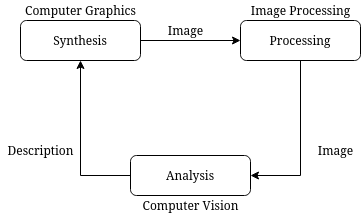
\includegraphics[width=.55\textwidth]{cycle.png}
    \caption{Visual Computing Cycle}
    \label{fig:cycle}
\end{figure}
Although they are different areas with their own sets of algorithms, they interact with each other, they are all related to images and share some techniques. Some applications need more than one of these areas to be achieved.

Visualization can interact with every other mentioned area, for example in descriptions. It utilizes graphics to better display data for analysis.

% %%%%%%%%%%%%%%%%%%%
\section*{Question 2}
% %%%%%%%%%%%%%%%%%%%
{\bfseries Is it correct to say that the Artificial Vision area depends on the Image Processing area?  Justify your answer.}

Computer Vision can depend on Image Processing for obtaining better results and, therefore, depends on it in most applications. Processing is important for various reasons, such as extracting the important information from the image (borders of objects, for example) or improving contrast/brightness so that it's easier to identify what is needed. Depending on the image acquired and the problem, it can be almost impossible to solve without first processing the image to receive better input.

% %%%%%%%%%%%%%%%%%%%
\section*{Question 3}
% %%%%%%%%%%%%%%%%%%%
{\bfseries What are the basic steps of a typical Artificial Vision system?  Briefly describe each of these steps.}

An Artificial Vision system starts with the \textbf{acquisition} of an image with a digital camera or other device, representing the scene to be "seen". Then, that image can be \textbf{pre-processed} in its entirety, to improve the quality of the input, which leads to the \textbf{processing} phase, when only the important information for the application is filtered and cleared for better analysis (for example, extracting borders of objects and filtering noise).

This image passes then through \textbf{analysis}, which depends on the application at hand (for example, identifying bifurcations and terminals in fingerprints). These points of interest are then modeled through \textbf{feature extraction} (for example, combining multiple identified points geometrically) and then finally used for \textbf{pattern recognition} by comparing the final structure with previous inputs or a stored reference.

% %%%%%%%%%%%%%%%%%%%
\section*{Question 4}
% %%%%%%%%%%%%%%%%%%%
{\bfseries What is the main difference between applications of Scientific Visualization and Information Visualization?  Give examples of each.}

The main difference between both fields of visualization are in the subject of visualization. While Scientific Visualization is used for modeling something that exists in the real world, Information Visualization is used for exploring raw data, often discrete and usually very abstract, therefore hard to comprehend without projection.

Scientific Visualization can cover models of the human brain or body, physics concepts such as wave propagation and quantum tunneling, chemical reactions and models or a human biological cell. Information Visualization, on the other hand, can be used to represent \textit{n-dimensional} spaces through projection in 3-D or 2-D (in machine learning, for example) or image histograms.

\end{document}